%%%%%%%%%%%%%%%%%%%%%%%%%%%%%%%%%%%%%%%%%%%%%%%%%%%%%%%%%%%%%%%%%%%%%%%%%%%%%%%%
%2345678901234567890123456789012345678901234567890123456789012345678901234567890
%        1         2         3         4         5         6         7         8

\documentclass[letterpaper, 10 pt, conference]{ieeeconf}  % Comment this line out if you need a4paper

%\documentclass[a4paper, 10pt, conference]{ieeeconf}      % Use this line for a4 paper

\IEEEoverridecommandlockouts                              % This command is only needed if 
                                                          % you want to use the \thanks command

\overrideIEEEmargins                                      % Needed to meet printer requirements.

% See the \addtolength command later in the file to balance the column lengths
% on the last page of the document

% The following packages can be found on http:\\www.ctan.org
\usepackage{graphics} % for pdf, bitmapped graphics files
\usepackage{epsfig} % for postscript graphics files
%\usepackage{mathptmx} % assumes new font selection scheme installed
%\usepackage{times} % assumes new font selection scheme installed
\usepackage{amsmath} % assumes amsmath package installed
\usepackage{amssymb}  % assumes amsmath package installed
\usepackage{graphicx}
\usepackage{url}

\usepackage{xcolor}

\bibliographystyle{IEEEtran}
\graphicspath{ {images/} }
\newtheorem{theorem}{Theorem}
\newtheorem{corollary}{Corollary}
\newtheorem{lemma}{Lemma}
\newtheorem{remark}{Remark}

\title{\LARGE \bf
A Risk-Sensitive Finite-Time Reachability Problem for Safety of Stochastic Dynamic Systems}

\author{Margaret P. Chapman$^{1}$, Jonathan P. Lacotte$^{2}$, Donggun Lee$^{3}$, Kevin Smith$^{4}$, Victoria Cheng$^{5}$,\\ 
Jaime Fernandez-Fisac$^{1}$, Aviv Tamar$^{1}$, Susmit Jha$^{6}$, Claire J. Tomlin$^{1}$% <-this % stops a space
\thanks{$^{1}$M.C., J.F., A.T., and C.T. are with the Department of Electrical Engineering and Computer Sciences, University of California, Berkeley, USA.
        {\tt\small chapmanm@berkeley.edu}}%
\thanks{$^{2}$J.L. is with the Department of Aeronautics and Astronautics, Stanford University, USA.
        }%
\thanks{$^{3}$D.L. is with the Department of Mechanical Engineering, University of California, Berkeley, USA.
        }%
\thanks{$^{4}$K.S. is with OptiRTC, Inc. and the Department of Civil and Environmental Engineering, Tufts University, USA.
        }%
\thanks{$^{5}$V.C. is with the Department of Civil and Environmental Engineering, University of California, Berkeley, USA.
        }%
\thanks{$^{6}$S.J. is with SRI International, Menlo Park, California, USA.
		}%
}

\begin{document}

\maketitle
\thispagestyle{empty}
\pagestyle{empty}

%%%%%%%%%%%%%%%%%%%%%%%%%%%%%%%%%%%%%%%%%%%%%%%%%%%%%%%%%%%%%%%%%%%%%%%%%%%%%%%%
\begin{abstract}
A classic reachability problem for safety of dynamic systems is to compute the set of initial states from which 
the state trajectory is guaranteed to stay inside a given constraint set over some time horizon. 
In this paper, we leverage existing theory of reachability analysis and risk measures 
to formulate a \textit{risk-sensitive} reachability problem for safety of stochastic dynamic systems under non-adversarial disturbances
over a finite time horizon.
We provide two key contributions to the reachability literature. 
First, our formulation quantifies the distance between the boundary of the constraint set and the state trajectory for a stochastic dynamic system.
In the literature, Hamilton-Jacobi (HJ) reachability methods quantify this distance for non-deterministic systems subject to adversarial disturbances, while
stochastic reachability methods reduce the distance to a binary random variable in order to quantify the probability of safety. 
Second, our formulation accounts for rare high-consequence events by posing the optimal control problem in terms of a risk measure, 
called \textit{Conditional Value-at-Risk} (CVaR).
HJ reachability assumes that high-consequence events occur always, which may yield overly conservative solutions in practice,
whereas stochastic reachability does not explicitly account for rare high-consequence events,
since the optimal control problem is posed in terms of the expectation operator.
We define a \textit{risk-sensitive safe set} as the set of initial states from which the risk of extreme constraint violations
can be made small via an appropriate control policy, where risk is quantified using CVaR.
We show that certain risk-sensitive safe sets enjoy probabilistic safety guarantees.
We provide a dynamic programming algorithm to compute under-approximations of risk-sensitive safe sets
and prove the correctness of the algorithm for finite probability spaces.
Our proof is a novel contribution, as it does not require the assumption of strong duality, which was required in a previous paper.
Finally, we demonstrate the utility of risk-sensitive reachability analysis on a numerical example.
%as a design tool for stormwater infrastructure which is required to operate safely in the presence of rainfall uncertainty.
\end{abstract}
% Premise (hypothesis): A description of the problem being addressed, and the basic idea to address it. For an applications article, this would be a description of what the application was designed to do.
% Process (experiments): A description of what the authors actually did. For an application article, this would be the detail of the application itself; for a design article, the thought process that went in to the design.
% Outcome (results): What the experiment produced, or how the application performed, or the final design (for a design article).
% Conclusion: A summary of the lessons learned from the paper.
%%%%%%%%%%%%%%%%%%%%%%%%%%%%%%%%%%%%%%%%%%%%%%%%%%%%%%%%%%%%%%%%%%%%%%%%%%%%%%%%
\section{Introduction}
Reachability analysis is a formal verification method based on optimal control theory that is used to prove 
safety or performance properties of dynamic systems~\cite{bansal2017hamilton}.
A classic reachability problem for safety is to compute the set of initial states from which 
the state trajectory is guaranteed to stay inside a given constraint set over some time horizon.
This problem was first considered for discrete-time dynamic systems by Bertsekas and Rhodes 
under the assumption that disturbances are uncertain but belong to known sets~\cite{bertsekas1971control},~\cite{bertsekas1971minimax},~\cite{bertsekas2005dynamic}.
In this context, the problem is solved using a minimax formulation,
in which disturbances behave adversarially and safety is described as a binary notion based on set membership~\cite{bertsekas1971control},~\cite{bertsekas1971minimax},~\cite{bertsekas2005dynamic}.\footnotemark 
\footnotetext{in ref.~\cite{bertsekas2005dynamic}, see Sec. 3.6.2, ``Control within a Target Tube"}

In practice, minimax formulations can yield overly conservative solutions, particularly because disturbances are not often adversarial.
Most storms do not cause major floods, and most vehicles are not involved in pursuit-evader games.
If there are enough observations of the system, one can estimate a probability distribution
for the disturbance, and then assess safety properties of the system in a more realistic context.\footnotemark
\footnotetext{Ref.~\cite{silverman2018density} presents methods for estimating probability distributions.} 
For stochastic discrete-time dynamic systems, %Assuming that a probabilistic discrete-time dynamics model is available, 
Abate et al. developed an algorithm that computes the set of initial states
from which the probability of safety of the state trajectory can be made large by an appropriate control policy~\cite{abate2008probabilistic}.\footnotemark
\footnotetext{Safety of the state trajectory is the event that the state trajectory stays in the constraint set over a finite time horizon.} 
Summers and Lygeros extended the algorithm of Abate et al. to quantify the probability of safety and performance
of the state trajectory, by specifying that the state trajectory should also reach a target set~\cite{summers2010verification}.   

Both the stochastic reachability methods~\cite{abate2008probabilistic},~\cite{summers2010verification} and the minimax reachability methods~\cite{bertsekas1971control},~\cite{bertsekas1971minimax},~\cite{bertsekas2005dynamic} for discrete-time dynamic systems
describe safety as a binary notion based on set membership.
In Abate et al., for example, the probability of safety to be optimized is the expectation of the product (or maximum)
of indicator functions, where each indicator encodes the event that the state at a particular time point is inside a given set~\cite{abate2008probabilistic}.
The stochastic reachability methods~\cite{abate2008probabilistic},~\cite{summers2010verification} 
do not generalize to quantify the random distance between the state trajectory and the boundary of the constraint set,
since they use indicator functions to convert probabilities to expectations to be optimized.

In contrast, Hamilton-Jacobi (HJ) reachability methods quantify the deterministic analogue of this distance
for continuous-time systems subject to adversarial disturbances 
(e.g., see~\cite{bansal2017hamilton},~\cite{herbert2017fastrack},~\cite{EECS-2018-41},~\cite{mitchell2005toolbox}).
Quantifying the distance between the state trajectory and the boundary of the constraint set in a non-binary fashion
may be important in applications where the boundary is not known exactly,
or where mild constraint violations are inevitable, but extreme constraint violations must be avoided.

It is imperative that reachability methods for safety take into account the possibility that rare events can occur
with potentially damaging consequences. 
Reachability methods that assume adversarial disturbances (e.g.,~\cite{bansal2017hamilton},~\cite{bertsekas1971minimax}) suppose that harmful events can always occur,
which may yield solutions with limited practical utility, especially in applications with large uncertainty sets.
Stochastic reachability methods~\cite{abate2008probabilistic},~\cite{summers2010verification} do not explicitly account for rare high-consequence events
because the optimal control problem is expressed as an expectation. 

In contrast, we leverage existing results on \textit{risk measures} to formulate an optimal control problem
that explicitly encodes a realistic viewpoint on the possibility of rare high-consequence events: 
harmful events are likely to occur at some point, but they are unlikely to occur always.
A \textit{risk measure} is a function that maps a random variable, $Z$, representing loss into the real line,
according to the risk associated with $Z$ (see~\cite{shapiro2009lectures}, Sec. 6.3; see~\cite{kisiala2015conditional}, Sec. 2.2).
Risk-sensitive optimization
is being studied in applied mathematics~\cite{ruszczynski2010risk}, reinforcement learning~\cite{osogami2012robustness},~\cite{chow2015risk},~\cite{ratliff2017risk}, and optimal control~\cite{chow2014framework}.\footnotemark
\footnotetext{In risk-sensitive optimization, the risk of a cost is minimized, where risk is quantified using a risk measure.
Conversely, in stochastic optimization, we usually minimize the expected value of a cost.} 
Risk-sensitive formulations have the potential to inform practical decision-making that also protects
against damaging outcomes~\cite{serraino2013conditional}, where the level of conservatism can be modified as needed.
%~\cite{serraino2013conditional} says "Cvar protects against outcomes that hurt the most", do i need citation in the sentence above?

We use a particular risk measure, called \textit{Conditional Value-at-Risk} (CVaR), in this paper.
If $Z$ is a random cost with finite expectation, then the Conditional Value-of-Risk of $Z$ at confidence level $\alpha \in (0,1)$
is, 
\begin{equation}
\text{CVaR}_\alpha[Z] = {\underset{t \in \mathbb{R}}\min} \text{ }\Big\{ t + \frac{1}{\alpha}\mathbb{E}\big[\max\{Z-t,0\}\big] \Big\};
\label{cvareqn}
\end{equation}
see~\cite{shapiro2009lectures}, Equation 6.22.\footnotemark
\footnotetext{Conditional Value-at-Risk is also called \textit{Average Value-at-Risk}, which is abbreviated as AV@R in~\cite{shapiro2009lectures}.}
Note that $\text{CVaR}_\alpha[Z]$ increases from $\mathbb{E}[Z]$ to $\sup Z$, as $\alpha$ decreases from 1 to 0.\footnotemark
\footnotetext{Technically, $\text{CVaR}_\alpha[Z] \rightarrow \text{ess}\sup Z$ as $\alpha \rightarrow 0$, 
where $\text{ess}\sup Z$ is the \textit{essential supremum} of $Z$. Informally, essential supremum is a supremum for random variables.}
Further, there is a well-established relationship between CVaR and chance constraints
that we use to obtain probabilistic safety guarantees. 
Chow et al. provides tractable methods to compute the CVaR of a cumulative cost
incurred by a Markov Decision Process~\cite{chow2015risk} that we also leverage.
CVaR has additional desirable properties that are of particular interest to researchers in financial risk management and are summarized in ref.~\cite{serraino2013conditional}. 

The key contributions of this paper follow.
We formulate a risk-sensitive reachability problem for safety of stochastic dynamic systems under non-adversarial disturbances
over a finite time horizon. In particular, our formulation quantifies the non-binary distance between the boundary of the constraint set and the
state trajectory for a stochastic dynamic system. This is an extension of stochastic 
reachability methods (e.g.,~\cite{abate2008probabilistic},~\cite{summers2010verification}), which reduce this distance to a binary random variable.
Further, in contrast to stochastic reachability methods, our formulation explicitly accounts for rare high-consequence events by posing the optimal control problem
in terms of Conditional Value-at-Risk instead of expectation. This is the first use of risk measures in the reachability literature to our knowledge.
In Sec.~\ref{problem}, we define the notion of a \textit{risk-sensitive safe set} and formalize the problem statement.
Sec.~\ref{prop} summarizes properties of risk-sensitive safe sets, including their relation to probabilistic safety.
Sec.~\ref{alg} provides a dynamic programming algorithm to compute under-approximations of risk-sensitive safe sets. %include proof?
In Sec.~\ref{ex}, we provide a numerical example in the context of the design of stormwater infrastructure. Sec.~\ref{conc} provides steps for future work.
% Extends upon HJ Reachability analysis~\cite{mitchell2005time}, \cite{bansal2017hamilton} - quantifies distance but for stochastic dynamic systems.

\section{Problem Statement}\label{problem}
We consider a stochastic discrete-time dynamic system over a finite time horizon,\footnotemark
\footnotetext{The system model is a special case of the model given by~\cite{bertsekas2005dynamic} in Sec. 1.2.}
\begin{equation}
x_{k+1} = f(x_k,u_k,w_k), \text{ }\text{ } k = 0, 1, \dots, N-1,
\label{sys}\end{equation}
such that $x_k \in \mathbb{R}^n$ is the state of the system at time $k$,
$u_k \in U$ is the control at time $k$, and
$w_k \in D$ is the random disturbance at time $k$. $U$ and $D$ are finite sets of real-valued vectors.
The dynamics function, $f : \mathbb{R}^n \times U \times D \rightarrow \mathbb{R}^n$, is bounded and Lipschitz continuous.
The probability that the disturbance equals $d_j \in D$ at time $k$ is, $\mathbb{P}[w_k = d_j] = p_j$, 
where $0 \leq p_j \leq 1$ and $\sum_{j=1}^W p_j = 1$.\footnotemark
\footnotetext{We also assume that $w_k$ is independent of $x_k$, $u_k$, and disturbances at any other times.}  
The only source of randomness in the system is the disturbance. The controls are not random.
The initial condition, $x_0$, is not random. 
The states, $(x_1, \dots, x_N)$, are random because they depend on the random disturbance. 
The collection of \textit{admissible control policies} is,
\begin{equation}
\Pi := \big\{ (\mu_0, \mu_1, \dots, \mu_{N-1}), \text{ where } \mu_k: \mathbb{R}^n \rightarrow U \big\}.
\label{pi}
\end{equation}

We are given a constraint set, $\mathcal{K} \subset \mathbb{R}^n$, and the safety criterion that 
the state of the system should stay inside $\mathcal{K}$ over time. 
For example, if the system is a pond, then $x_k$ may be the water level of the pond at time $k$,
and $\mathcal{K} := [0, 5\text{ft})$ indicates that the pond overflows if the water level exceeds 5ft.
We quantify the extent of constraint violation/satisfaction using a surface function that characterizes the constraint set.
Let $g: \mathbb{R}^n \rightarrow \mathbb{R}$ satisfy,
\begin{equation}
x \in \mathcal{K} \iff g(x) < 0,
\label{g}
\end{equation}
where we adopt the convention provided by~\cite{EECS-2018-41} in Equation 2.3.
For example, we may choose $g(x) := x - 5$ to characterize $\mathcal{K} := [0, 5\text{ft})$ on the state space, 
$\mathbb{R}_+ := [0, \infty)$.

We define a \textit{risk-sensitive safe set} as a set of initial states from which 
risk of extreme constraint violation over time can be made small using an admissible control policy~\eqref{pi}, where risk is quantified by \textit{Conditional Value-at-Risk}~\eqref{cvareqn}.
Formally, the risk-sensitive safe set at the confidence level, $\alpha \in (0,1)$, and the risk level, $r \in \mathbb{R}$, is defined as,
\begin{subequations}\label{myS}
\begin{equation}
\mathcal{S}_\alpha^r := \{x \in \mathbb{R}^n \mid W_0^*(x,\alpha) < r \}, \\
\end{equation}
where 
\begin{equation}\begin{aligned}
& W_0^*(x,\alpha) := {\underset{\pi \in \Pi}\inf} \text{ CVaR}_\alpha\big[ Z^\pi_{x} \big], \\
& Z^\pi_{x} := \max \big\{ g(x_k) \mid k = 0, \dots, N \big\},
\end{aligned}\end{equation}
\end{subequations}
such that the state trajectory $(x_0, x_1, ..., x_N)$
evolves according to the dynamics model~\eqref{sys} with the initial state, $x_0 := x$, under the admissible policy, $\pi \in \Pi$.
Note that $g$ characterizes the constraint set, $\mathcal{K}$, according to~\eqref{g}.
The goal of this paper is to compute a family of risk-sensitive safe sets at different levels of confidence, $\alpha \in (0,1)$, and risk, $r \in \mathbb{R}$.

\section{Rationale}
Computing risk-sensitive safe sets is a well-motivated problem for several reasons. 
\textcolor{blue}{This problem is more general than the stochastic reachability problem that is addressed by Abate et al.~\cite{abate2008probabilistic}.
Abate et al. solves for the \textit{maximal probabilistic safe set} at any safety level, $\epsilon \in [0, 1]$,
\begin{subequations}\label{abateS}
\begin{equation}
S^*(\epsilon) = \{ x \mid {\underset{\pi \in \Pi}\inf}\text{ }\mathbb{E}[ Q_x^\pi ] \leq \epsilon \},
\end{equation}
where
\begin{equation}
Q_x^\pi := \max \big\{ \textbf{1}_\mathcal{\bar{K}}(x_k) \mid k = 0,\dots, N \big\},
\end{equation}
such that the state trajectory $(x_0, x_1, ..., x_N)$ evolves according to a hybrid dynamics model with the initial state, $x_0 := x$,
under the admissible policy, $\pi \in \Pi$, and 
\begin{equation}
\textbf{1}_\mathcal{\bar{K}}(x) := \begin{cases} 1 \text{ if } x \notin \mathcal{K} \\ 0 \text{ if } x \in \mathcal{K} \end{cases};
\end{equation}
\end{subequations}
see~\cite{abate2008probabilistic}, Equations 11 and 13. 
If we choose $\alpha := 1$, $g(x) := \textbf{1}_\mathcal{\bar{K}}(x) - \frac{1}{2}$, and $r:= \epsilon-\frac{1}{2}$ in~\eqref{myS},
then we can compute~\eqref{abateS}. [Do you agree? What about the non-strict inequality in $S^*(\epsilon)$? 
What is the difference between the set of Markov policies $\mathcal{M}_m$ in Abate, and our $\Pi$? 
Abate did his formulation for hybrid systems, but we are not doing this explicitly]} 

Further, risk-sensitive safe sets have two desirable mathematical properties.
The first property is that $\mathcal{S}_\alpha^r$ shrinks as the risk level, $r$, or the confidence level, $\alpha$, decrease.
Since $\mathcal{S}_\alpha^r$ is an $r$-sublevel set and $\text{CVaR}_\alpha$ increases as $\alpha$ decreases,
one can show that,
\begin{equation}\begin{aligned}
& \mathcal{S}_{\alpha_2}^{r_2} \subseteq \mathcal{S}_{\alpha_1}^{r_2} \subseteq \mathcal{S}_{\alpha_1}^{r_1}, \text{ and } \\
& \mathcal{S}_{\alpha_2}^{r_2} \subseteq \mathcal{S}_{\alpha_2}^{r_1} \subseteq \mathcal{S}_{\alpha_1}^{r_1}
\end{aligned}\end{equation}
hold for any $r_1 \geq r_2$ and $1 > \alpha_1 \geq \alpha_2 > 0$.
In other words, as the allowable level of risk of constraint violation ($r$) decreases, or
\textcolor{blue}{as the fraction of damaging outcomes that are not fully addressed ($\alpha$) decreases},
$\mathcal{S}_\alpha^r$ encodes a higher degree of safety.

The second property is that the risk-sensitive safe sets at risk level, $r := 0$, enjoy probabilistic safety guarantees.
\begin{lemma}\label{mylemma1}
If $x \in \mathcal{S}_\alpha^0$, then the probability that the state trajectory initialized at $x$ exits the constraint set can be made strictly
less than $\alpha$ by an admissible control policy.
\end{lemma}
\begin{proof}
The proof follows from the fact,\footnotemark \\
\footnotetext{The constraint, $\text{CVaR}_\alpha[Z] \leq 0$, gives a conservative approximation of the chance constraint, $\mathbb{P}[Z > 0] \leq \alpha$,
for any random variable $Z$ with finite expectation (see~\cite{shapiro2009lectures}, Sec. 6.2.4).
We do not show $\text{CVaR}_\alpha[Z] < 0 \implies \mathbb{P}[Z\geq 0] < \alpha$ for brevity.} %pp. 257-258
$\text{CVaR}_\alpha[Z_x^\pi] < 0 \implies \mathbb{P}[Z_x^\pi\geq 0] < \alpha$. \\
Further, the event, $Z_x^\pi\geq 0$, is equivalent to the event that there exists a state, $x_k$, of the associated trajectory 
that exits the constraint set, since $g(x) \geq 0 \iff x \notin \mathcal{K}$.\footnotemark
\footnotetext{``Associated trajectory" refers to the trajectory that is initialized at $x$ and evolves under the policy, $\pi \in \Pi$,
according to the dynamics model~\eqref{sys}.}
\end{proof}
\begin{remark}{}
Lemma~\ref{mylemma1} indicates that $\mathcal{S}_\alpha^0$ is a subset of Abate et al.'s \textit{maximal probabilistic safe set} at the safety level, $\alpha$;
see~\cite{abate2008probabilistic}, Equations 9 and 11.
\end{remark}

\section{Computational Method}\label{alg}
The computation of risk-sensitive safe sets is challenging due to the presence of the maximum of costs (as opposed to a summation of costs)
and the use of Conditional Value-at-Risk (as opposed to an expectation). In this paper, we provide under-approximations 
for risk-sensitive safe sets, and an algorithm to compute these under-approximations. Define $\mathcal{U}_\alpha^r$
for the confidence level, $\alpha \in (0,1)$, and the risk level, $r \in \mathbb{R}$,
\begin{subequations}\label{under}\begin{equation}
\mathcal{U}_\alpha^r := \{x \in \mathbb{R}^n \mid J_0^*(x,\alpha) < \beta e^{m\cdot r} \},
\end{equation}
where
\begin{equation}\begin{aligned}
& J_0^*(x,\alpha) := {\underset{\pi \in \Pi}\inf} \text{ CVaR}_\alpha \big[ Y_x^\pi \big],\\
& Y_x^\pi := \textstyle\sum_{k=0}^N \beta e^{m\cdot g(x_k)},
\end{aligned}\end{equation}
\end{subequations}
such that the state trajectory $(x_0, x_1, ..., x_N)$
satisfies~\eqref{sys} with the initial state, $x_0 := x$, under the policy, $\pi \in \Pi$;
$\beta > 0$ and $m > 0$ are constants.
\begin{lemma}\label{lemma2}
$\mathcal{U}_\alpha^r$ is a subset of the risk-sensitive set, $\mathcal{S}_\alpha^r$. 
Also, the gap between $\mathcal{U}_\alpha^r$ and $\mathcal{S}_\alpha^r$ can be made smaller by increasing $m$.
\end{lemma}
\begin{proof}
The proof relies on two facts. The first fact is,
\begin{equation}\begin{aligned}
\max\{x_1, \dots, x_p\} & \leq \log( e^{x_1}+ \dots +e^{x_p} ) \\
						& \leq \max\{x_1, \dots, x_p\} + \log p,
\end{aligned}\end{equation}
for any $x \in \mathbb{R}^p$; see~\cite{boyd2004convex}, Sec. 3.1.5 Examples.
Using this fact, one can show the following,
\begin{subequations}\label{related}
\begin{equation}\begin{aligned}
\max\{y_1, \dots, y_p\} & \leq \frac{1}{m}\log( e^{my_1}+ \dots +e^{my_p} ) \\
						& \leq \max\{y_1, \dots, y_p\} + \frac{\log p}{m},
\end{aligned}\end{equation}
for any $y \in \mathbb{R}^p$, $m > 0$. So, as $m \rightarrow \infty$,
\begin{equation}
\frac{1}{m}\log( e^{my_1}+ \dots +e^{my_p} ) \rightarrow \max\{y_1, \dots, y_p\}.
\end{equation}
\end{subequations}
The second fact is that Conditional Value-at-Risk is a \textit{coherent risk measure},
so it satisfies useful properties. 
In particular, CVaR is positively homogeneous,
$$\text{CVaR}_\alpha[\lambda Z] = \lambda\text{CVaR}_\alpha[Z],$$ 
for any $\lambda \geq 0$ and random variable $Z$,
and monotonic,
$$\text{CVaR}_\alpha[Y] \leq \text{CVaR}_\alpha[Z],$$
for any random variables, $Y \leq Z$; see~\cite{kisiala2015conditional}, Sec. 2.2.
Further, CVaR can be expressed as the supremum expectation over a particular set of probability density functions;
see~\cite{shapiro2009lectures}, Equations 6.40 and 6.70.
Using this property and the fact, $\mathbb{E}[\log(Z)] \leq \log \left(\mathbb{E}[Z]\right)$,
one can show,
\begin{equation}
\text{CVaR}_\alpha[\log(Z)] \leq \log \left(\text{CVaR}_\alpha[Z]\right),
\label{logeq}\end{equation}
for any random variable, $Z$, with finite expectation.
By monotonicity, positive homogeneity,~\eqref{related}, and~\eqref{logeq},
\begin{equation}\begin{aligned}
\text{CVaR}_\alpha\big[ Z_x^\pi \big] & \leq \frac{1}{m} \text{CVaR}_\alpha\big[ \log\left( Y_x^\pi/\beta \right) \big] \\
& \leq \frac{1}{m} \log \left(\text{CVaR}_\alpha\big[ Y_x^\pi/\beta \big] \right).
\end{aligned}\label{12}\end{equation}
If $x \in \mathcal{U}_\alpha^r$, then $\exists \pi \in \Pi$ such that,\footnotemark
\begin{equation*}\begin{aligned}
& \text{CVaR}_\alpha \big[ Y_x^\pi /\beta \big] < e^{m\cdot r} \iff \frac{1}{m}\log \left( \text{CVaR}_\alpha \big[  Y_x^\pi /\beta \big] \right) < r \\
& \implies \text{CVaR}_\alpha\big[ Z_x^\pi \big] < r, \\
\end{aligned}\end{equation*}
\footnotetext{The minimum is attained because the random variables in this paper have finite expectation.} 
where the last line holds by~\eqref{12}. So, $x \in \mathcal{S}_\alpha^r$.
\end{proof}
\begin{remark}
$\beta$ is included in~\eqref{under} to help counter numerical issues that may arise if $m$ is chosen very large.
\end{remark}

Next, we provide an algorithm to compute the under-approximation, $\mathcal{U}_\alpha^r$,
at different levels of confidence and risk, that is based on insights by Chow et al.~\cite{chow2015risk}.
\subsection{Algorithm}
The value function, $J_0^*(x,\alpha)$, defined in~\eqref{under},
is the smallest risk at the confidence level, $\alpha$, of the cumulative scaled constraint violation of the state trajectory that satisfies~\eqref{sys} with $x_0 := x$.
This value function can be computed by considering 
an observable \textit{augmented state}, $(x,\alpha)$, that consists of the original state and the confidence level,
and the augmented set of control policies,
\begin{equation}\begin{aligned}
& \bar{\Pi}_k := \{ (\mu_k, \mu_{k+1}, \dots, \mu_{N-1}), \mu_i: \mathbb{R}^n \times (0,1) \rightarrow U \},\\
& k = 0, \dots, N-1.
\end{aligned}\label{augpi}\end{equation}
In particular, the following equality holds,
\begin{equation}
J_0^*(x,\alpha) = {\underset{\pi \in \bar{\Pi}_0}\inf} \text{ CVaR}_\alpha \Big[ \textstyle\sum_{k=0}^N \beta e^{m g(x_k)} \Big],
\label{J0}
\end{equation}
where the optimization is over the augmented policy space.
We provide an algorithm that computes the right-hand-side of~\eqref{J0}.
The algorithm is based on a prior result that provides the dynamics of the confidence level.
Subsequently, we let $c: \mathbb{R}^n \rightarrow \mathbb{R}$ be any stage cost; e.g., $c(x) = \beta e^{m g(x)}$ in~\eqref{J0}.  

\begin{lemma}\label{decomlemma}
Lemma 22 of~\cite{pflug2016time} implies the following CVaR-decomposition for the system~\eqref{sys} at time $k$,
under any (augmented) policy, $\pi_k := (\mu_k, \pi_{k+1}) \in \bar{\Pi}_k$,
\begin{subequations}\label{decomp}\begin{equation}\begin{aligned}
& \text{CVaR}_\alpha \Big[ Z \Big| x_k, \pi_k \Big] \\
& = {\underset{R \in \mathcal{R}(\alpha, \mathbb{P})}\max} \mathbb{E}\Big[ R \cdot \text{CVaR}_{\alpha R}\big[ Z \big| x_{k+1}, \pi_{k+1} \big] \Big| (x_k, \alpha), \mu_k \Big], \\
\end{aligned}\end{equation}
where 
\begin{equation}
\mathcal{R}(\alpha, \mathbb{P}) := \Bigg\{ R : D \rightarrow \big[0,\alpha^{-1}\big], \sum_{j=1}^W R(d_j)\mathbb{P}[w_k = d_j] = 1 \Bigg\}\\
\end{equation}\end{subequations}
is a set of discrete random variables, 
and $Z := \textstyle \sum_{i=k+1}^N c(x_i)$ is the random cumulative cost starting at time $k+1$.
\end{lemma}
\begin{remark}
The proof of Lemma~\ref{decomlemma}, which we do not provide due to lack of space, relies on the measure-theoretic definition of conditional expectation, and the fact that 
the system~\eqref{sys} is Markov. \textcolor{blue}{please provide more details here}
\end{remark}
\begin{remark}
$\text{CVaR}_\alpha \big[ \textstyle \sum_{i=k+1}^N c(x_i) \big| x_k, \pi_k \big]$ is the risk of 
the cumulative cost starting at time $k+1$ of the trajectory that starts at time $k$, is initialized at the state, $x_k \in \mathbb{R}^n$, 
and evolves under the policy, $\pi_k \in \bar{\Pi}_k$.
\end{remark}
\begin{remark}
For the system~\eqref{sys},
\begin{equation*}\begin{aligned}
& \mathbb{E}\Big[ R \cdot \text{CVaR}_{\alpha R}\big[ Z \big| x_{k+1}, \pi_{k+1} \big] \Big| (x_k, \alpha), \mu_k \Big] \\
& = \textstyle\sum_{j=1}^W v_j \cdot \text{CVaR}_{\alpha v_j}\big[ Z \big| x_{k+1}^j, \pi_{k+1} \big] \cdot \mathbb{P}[w_k = d_j]\text{, where}\\
& x_{k+1}^j = f(x_k, \mu_k(x_k, \alpha), d_j).
\end{aligned}\end{equation*}
In words, $x_{k+1}^j$ is the $j$\textsuperscript{th} sample of the state at time $k+1$, given the control at time $k$, $\mu_k(x_k, \alpha) \in U$, 
and the disturbance at time $k$, $w_k = d_j$.
Further, $v_j = R(d_j)$ is the $j$\textsuperscript{th} sample of the random variable, $R \in \mathcal{R}(\alpha, \mathbb{P})$. 
\end{remark}
\begin{remark}
Chow et al.~\cite{chow2015risk} interpreted Lemma 22 of~\cite{pflug2016time} for Markov Decision Processes.
Lemma~\ref{decomlemma} restates the result for stochastic dynamic systems.
\end{remark}

Next, we use Lemma~\ref{decomlemma} to provide a dynamic programming value-iteration that computes~\eqref{J0}.
\begin{theorem}\label{thm}
Define the functions, $J_{N-1}$, \dots, $J_0$, recursively as follows, $\forall (x_k, y_k) \in \mathbb{R}^n \times (0,1)$,
\begin{equation}\begin{aligned}
& J_k(x_k,y_k) := \\
& {\underset{u_k \in U}\min} \Bigg\{ c(x_k) + {\underset{R \in \mathcal{R}(y_k, \mathbb{P})}\max} \mathbb{E}\Big[ R J_{k+1}(x_{k+1}, y_k R) \Big| (x_k, y_k), u_k \Big] \Bigg\}, \\
& k = N-1, \dots, 0,
\end{aligned}\label{bell}\end{equation}
where $J_N(x_k, y_k) := c(x_k)$, $x_{k+1}$ satisfies~\eqref{sys}, and $\mathcal{R}(y_k, \mathbb{P})$ is defined in~\eqref{decomp}.  
Then, $J_0^*(x,\alpha)$, see~\eqref{J0}, is given by $J_0(x, \alpha)$, 
the value of the function at the last step of the recursion evaluated at $(x,\alpha) \in \mathbb{R}^n \times (0,1)$.
\end{theorem}
\begin{remark}
The functions, $J_{N-1}$, \dots, $J_0$, are well-defined and finite because $D$ is a finite set (see~\cite{bertsekas2005dynamic}, Sec. 1.5).
\end{remark}
\begin{remark}
Chow et al. proposed the recursion~\eqref{bell} and applied it to the infinite-time discounted problem~\cite{chow2015risk}. 
The part of their proof that addresses the finite time case assumes that the min/max can be exchanged (see~\cite{chow2015risk}, Theorem 4),
which our proof does not assume. 
\end{remark}

Our proof of Theorem~\ref{thm} is provided in the Appendix.
The idea is to use a sub-optimal value function as machinery to demonstrate that each $J_k$, as defined recursively in~\eqref{bell},
is sufficiently close to the optimal cost-to-go of the sub-problem that starts at time $k$,
\begin{equation}
J_k^*(x_k, y_k) := {\underset{\pi_k \in \bar{\Pi}_k}\min} \text{ CVaR}_{y_k} \Big[ \textstyle\sum_{i=k}^N c(x_i) \Big| (x_k, y_k), \pi_k \Big],
\end{equation}
via induction. This technique is also used to prove the suitability of the classic finite-time dynamic programming algorithm, 
where the value function is the expected cumulative cost (see~\cite{bertsekas2005dynamic}, Sec. 1.5).
We recommend the reader to review this proof before proceeding to ours. 

In this paper, we do not explicitly construct an optimal policy for practical use.
This is an important step for future work and may require different arguments 
than those used by~\cite{chow2015risk} (see Theorem 5). In particular, this policy would likely depend 
on the history of the states and the initial confidence level. However, the policy given by the algorithm~\eqref{bell}
requires the availability of the current state and the current confidence level. 
This subtle distinction deserves careful study that is out of scope of the current paper.

\section{Numerical Example}\label{ex}
We demonstrate the utility of computing approximate risk-sensitive safe sets on a practical example:
to evaluate the design of a stormwater retention pond. 
Stormwater management facilities, such as retention ponds, are required to operate safely 
in the presence of precipitation uncertainty, but must be designed within the scope of public resources (e.g., money, land). 
Standard design practices assess how empty ponds respond to a given \textit{design storm},
which is a synthetic storm based on historical rainfall.  
In our prior work, we proposed using reachability analysis to augment existing design practices, as it can assess 
system behavior from a larger number of initial conditions, but we treated the surface runoff generated by the design storm as a deterministic input~\cite{sustech}.
Here we consider the first pond from the example in our prior work as a stochastic discrete-time dynamic system,
\begin{equation}\begin{aligned}
& x_{k+1} = x_k + \frac{\triangle t}{A} (w_k - q_p(x_k, u_k)), \text{ }k = 0, \dots, N-1, \\
& q_p(x_k,u_k) := \begin{cases} C_d \pi r^2 u_k \sqrt{ 2\gamma(x-E) } & \text{ if } x_k \geq E \\
						0 & \text{ if } x_k < E, \end{cases}
\end{aligned}\label{watersys}\end{equation}
where $x_k \geq 0$ is the water level of the pond in feet at time $k$, $u_k \in \{0, 1\}$ is the valve setting at time $k$,
and $w_k \in D := \{d_1, \dots, d_{10}\}$ is the random surface runoff in feet-cubed-per-second at time $k$~\cite{sustech}.\footnotemark
\footnotetext{$\gamma = 32.2$ft/s\textsuperscript{2} is acceleration due to gravity, $\pi \approx 3.14$ is the usual constant, $r = 1/3$ft is the outlet radius, $A = 28,292$ft\textsuperscript{2} is the pond surface area, $C_d = 0.61$ is the discharge coefficient,
and $E = 1$ft is the elevation of the outlet. Some of the parameter names are changed from~\cite{sustech} to avoid abuse of notation.} 
We estimated a finite probability distribution for $w_k$ using the surface runoff samples that we previously generated from a time-varying design storm~\cite{sustech}. 
We averaged each sample over time and solved for a distribution
that satisfied the empirical statistics of the time-averaged samples (Table~\ref{dist}). 
We set $\triangle t := 300$ seconds, and $N := 48$ to yield a 4-hour horizon.
We set the constraint set, $\mathcal{K} := [0, 5\text{ft})$, and $g(x) := x - 5$.

\begin{table}
\begin{center}
\caption{}
\begin{tabular}{| p{3.5cm} | p{3.5cm} |}
\hline
\bf{Sample moment} & \bf{Value}  \\ \hline
Mean & 12.16 ft\textsuperscript{3}/s \\ 
Variance & 3.22 ft\textsuperscript{6}/s\textsuperscript{2} \\ 
Skewness & 1.68 ft\textsuperscript{9}/s\textsuperscript{3} \\ 
\hline 
\textbf{Disturbance sample}, $d_j$ ft\textsuperscript{3}/s & \textbf{Probability}, $\mathbb{P}[w_k = d_j]$ \\ \hline
$8.57$ 		& $0.0236$ \\
$9.47$ 		& $10^{-4}$ \\
$10.37$ 		& $10^{-4}$ \\
$11.26$  & $0.5249$ \\ 
$12.16$ & $0.3272$ \\ 
$13.06$  & $10^{-4}$ \\ 
$13.95$  & $10^{-4}$ \\ 
$14.85$  & $10^{-4}$ \\ 
$15.75$  & $10^{-4}$ \\ 
$16.65$  & $0.1237$ \\ \hline
\end{tabular}
\begin{flushleft} \end{flushleft}
\label{dist}
\end{center}
\end{table}

We computed risk-sensitive safe sets, $\{\mathcal{S}_y^r\}$~\eqref{myS}, using a Monte Carlo procedure 
and the under-approximations, $\{\mathcal{U}_y^r\}$~\eqref{under}, using the dynamic programming algorithm~\eqref{bell}.
The risk-sensitive sets and the under-approximations are shown for various confidence and risk levels in Fig.~\ref{compare}.
We performed the computations over a grid of states, $x \in G_s := \{0, 0.1\text{ft}, \dots, 6.4\text{ft}, 6.5\text{ft}\}$,
and confidence levels, $\alpha \in G_c := \{0.999, 0.95, 0.80, \dots, 0.20, 0.05, 0.001\}$; let $G = G_s \times G_c$.
Since the initial state, $x_0$, is non-negative and the smallest value of $w_k$ is about 8.5ft\textsuperscript{3}/s, 
$x_{k+1}\geq x_k$ for all $k$; see~\eqref{watersys} and Table~\ref{dist}. 
If $x_{k+1} > 6.5\text{ft}$ during our computations, we set $x_{k+1} := 6.5\text{ft}$ to stay within the grid.
All computations were done in MATLAB.\footnotemark 
\footnotetext{MATLAB R2016b, The MathWorks, Inc., Natick, MA}
Our code is available here~\cite{mycode}.

\textit{Dynamic programming implementation.}
To compute the under-approximations, $\{\mathcal{U}_y^r\}$, 
we solved for the value function, $J_0^*$, as expressed in~\eqref{J0},
using the value-iteration algorithm~\eqref{bell} over our grid, and then extracted the $\beta e^{m \cdot r}$-sublevel sets, see~\eqref{under}.
We used the interpolation method over the confidence levels proposed by Chow et al.~\cite{chow2015risk} 
to approximate the expectation in~\eqref{bell}
as a piecewise linear concave function, which we maximized by solving a linear program.\footnotemark
\footnotetext{The linear programs were solved using MOSEK (Copenhagen, Denmark) with CVX~\cite{grant2008cvx}.}
Further, we used multi-linear interpolation to approximate the value of $J_{k+1}(x_{k+1}, \alpha)$ at each $\alpha \in G_c$.
Although at step $k$ of the algorithm~\eqref{bell} the value of $J_{k+1}$ is known at each grid point,
$x_{k+1}$ is not necessarily in the grid, since the state space for the pond dynamics is continuous~\eqref{watersys}.
The function, $J_0$, generated by the algorithm~\eqref{bell}, is provided in Fig.~\ref{J0dp},
where $c(x) := \beta e^{m g(x)}$, $\beta := 10^{-3}$, $m := 10$, and $g(x):= x - 5$.
$J_0$ estimates $J_0^*$, which we expressed in~\eqref{J0} and originally defined in~\eqref{under}.  
The computation is inexact due to the interpolations over the grid.

\textit{Monte Carlo implementation.}
To compute the risk-sensitive safe sets, $\{\mathcal{S}_y^r\}$,
we solved for the value function, $W_0^*$, as defined in~\eqref{myS}, using a Monte Carlo procedure over our grid,
and then extracted the $r$-sublevel sets.
This computation is also inexact due to the nature of random sampling. 
The computational burden was manageable since an optimal control policy was known \textit{a priori}.
As $x_{k+1}\geq x_k$ for all $k$, and the only way to exit the constraint set is if $x_k \geq 5$ft,
the optimal control policy is to keep the valve open over time, regardless of the current state or confidence level.
For each $(x,\alpha) \in G$, we sampled 100,000 trajectories starting from $x_0 := x$, subject to keeping the valve open over time.
For each trajectory sample $i$, we computed the cost sample, $z_i := \max\{g(x_k^i)\}$, and estimated the Conditional Value-at-Risk
of the 100,000 cost samples at the confidence level, $\alpha$. 
We used the CVaR estimator, $\hat{\text{CVaR}}_\alpha[Z] := \frac{1}{\alpha M}\sum_{i=1}^M z_i \textbf{1}_{\{z_i\geq \hat{Q}_\alpha\}}$,
where $\hat{Q}_\alpha$ is the $(1-\alpha)$-quantile of the empirical distribution of the samples, $\{z_i\}_{i=1}^M$,
and $M := 100,000$ is the number of samples; see~\cite{shapiro2009lectures}, Sec. 6.5.1.
Since the estimator is designed for continuous distributions, which was not valid for every grid point,
we added zero-mean Gaussian noise with a small standard deviation ($\sigma := 10^{-12}$) to each cost sample prior to computing the CVaR.
The Monte Carlo estimate of $W_0^*$, as defined in~\eqref{myS}, is provided in Fig.~\ref{W0mc}.

One hundred thousand samples per grid point appears to be sufficient. We also used a Monte Carlo procedure to estimate $J_0^*$, see~\eqref{J0},
with 100,000 samples per grid point.\footnotemark
\footnotetext{We also added zero-mean Gaussian noise with a small standard deviation ($\sigma := 10^{-7}$)
to each cost sample prior to computing the CVaR. This standard deviation was chosen because the magnitude of $J_0$, see Fig.~\ref{J0dp}, is 
about $10^5$ times greater than the magnitude of $W_0$, see Fig.~\ref{W0mc}.}
The results of the Monte Carlo method, see Fig.~\ref{J0mc}, and the dynamic programming algorithm, see Fig.~\ref{J0dp}, are comparable
in most regions of the grid. The Monte Carlo procedure, however, does not capture the higher costs at the smallest level of confidence, $\alpha = 0.001$,
that are evident using the dynamic programming algorithm.   

\begin{figure}[thpb]
      \centering
      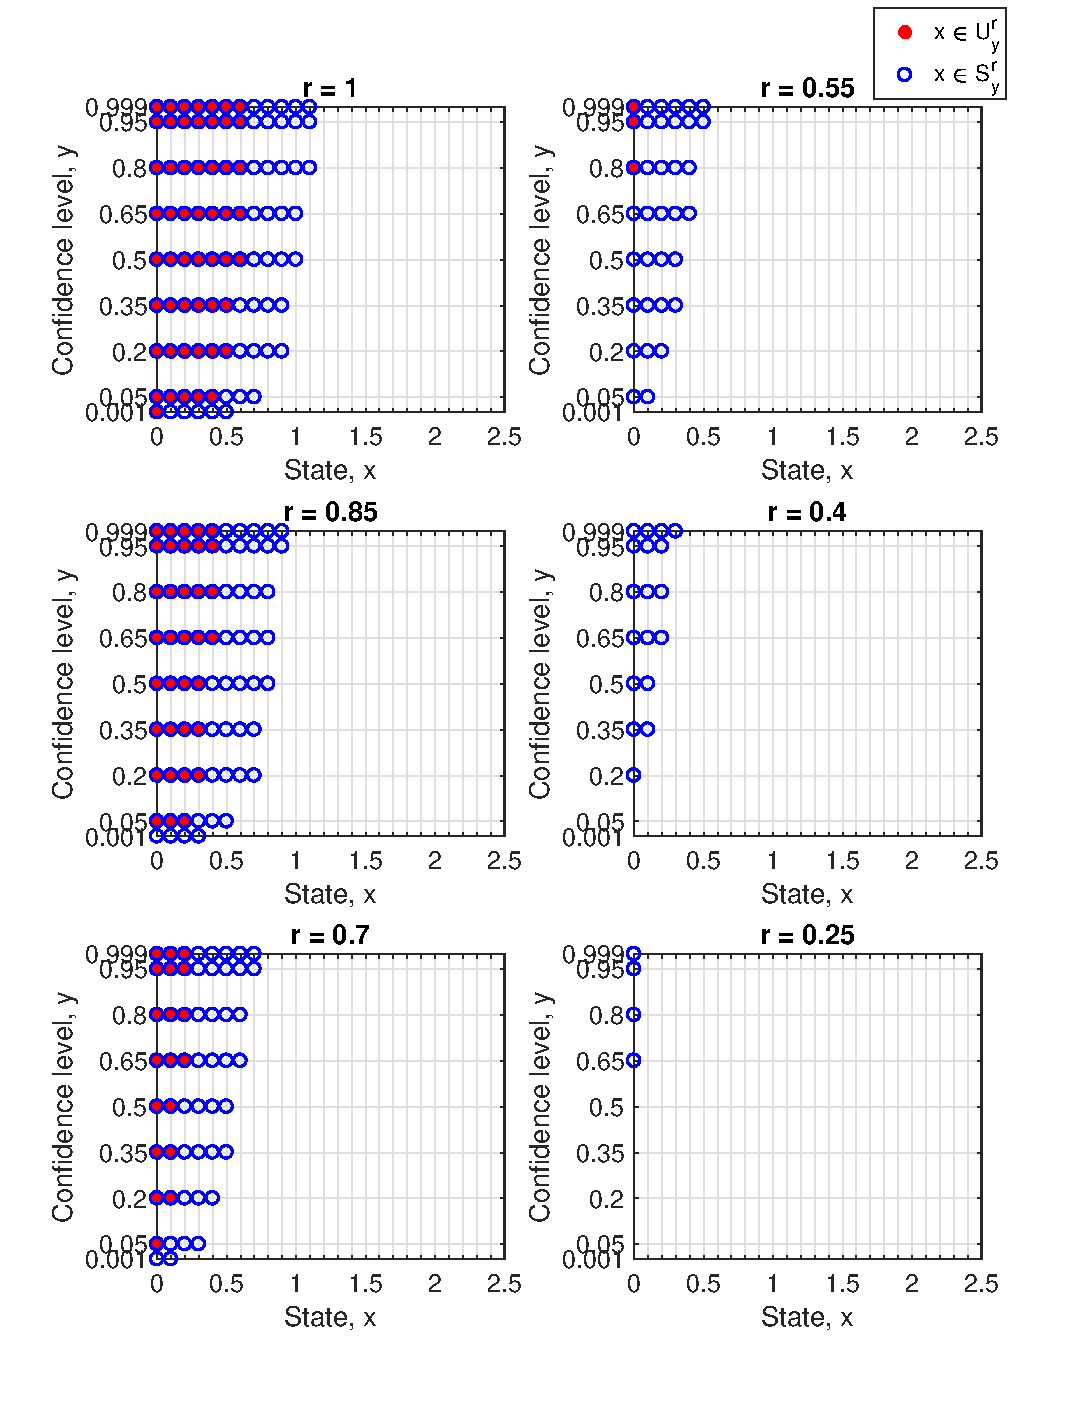
\includegraphics[scale=0.5]{output_CompareScript_Sept112018.pdf}
      \caption{ Risk-sensitive safe sets, $\mathcal{S}_y^r$~\eqref{myS}, and their under-approximations, $\mathcal{U}_y^r$~\eqref{under},
		are shown for various levels of confidence and risk. } 
      \label{compare}
\end{figure}

\begin{figure}[thpb]
      \centering
      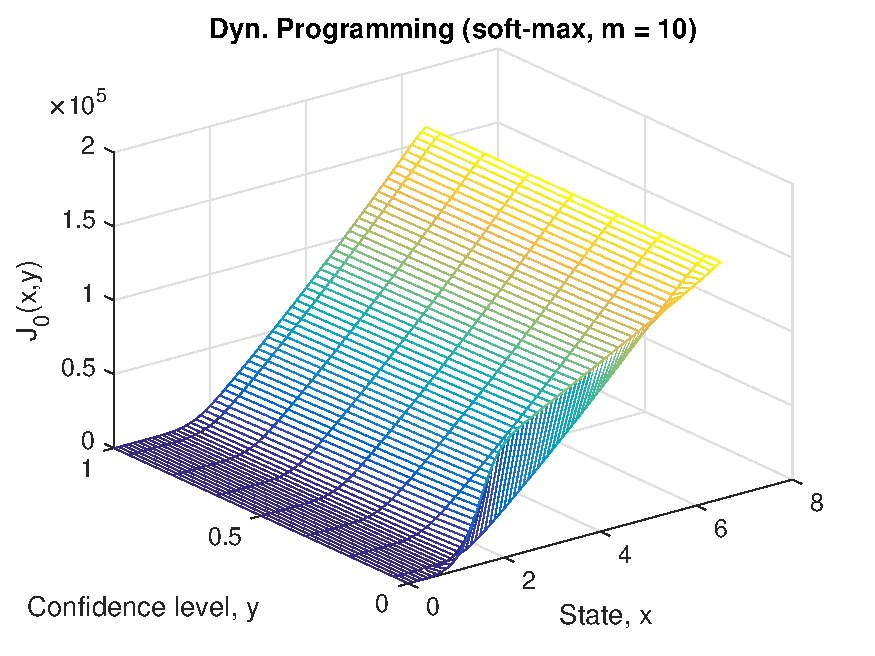
\includegraphics[scale=0.5]{dyn_prog_J0_sept112018.pdf}
      \caption{$J_0(x,\alpha)$ versus $(x, \alpha) \in G$ generated by the dynamic programming algorithm~\eqref{bell} for the pond system is shown.
	  $J_0$ estimates $J_0^*$, see~\eqref{J0}, where $c(x) := \beta e^{m g(x)}$, $\beta := 10^{-3}$, $m := 10$, $\mathcal{K} := [0, 5\text{ft})$, and $g(x) := x-5$.}
      \label{J0dp}
\end{figure}

\begin{figure}[thpb]
      \centering
      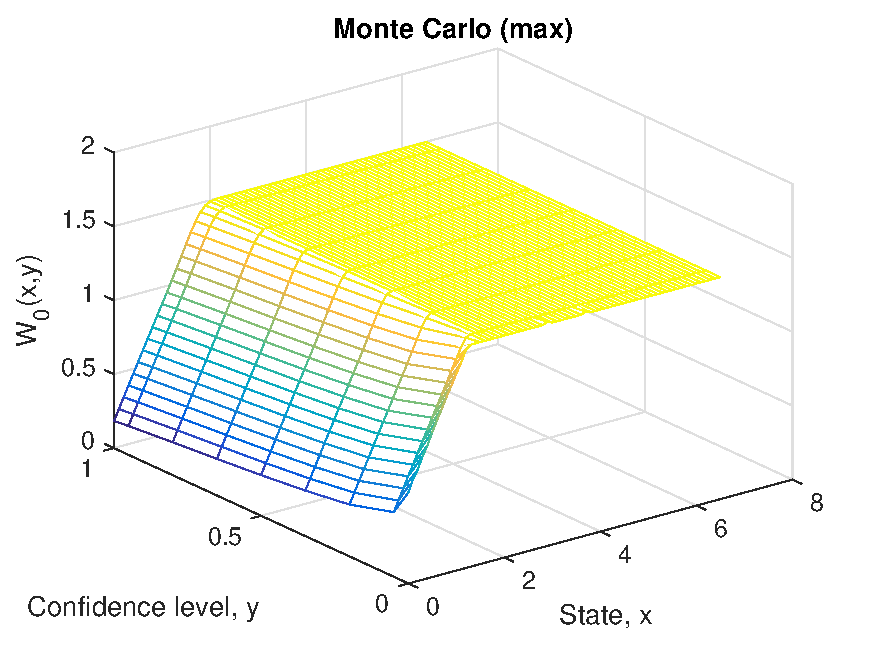
\includegraphics[scale=0.5]{monte_carlo_max_sept112018.pdf}
      \caption{A Monte Carlo estimate of $W_0^*(x,\alpha)$, as defined in~\eqref{myS}, versus $(x, \alpha) \in G$ is shown for the pond system.
	  100,000 samples were generated per grid point, $g(x) := x - 5$, and $\mathcal{K} := [0, 5\text{ft})$. 
	  The maximum is 1.5ft because the system state was prevented from exceeding 6.5ft.}
      \label{W0mc}
\end{figure}

\begin{figure}[thpb]
      \centering
      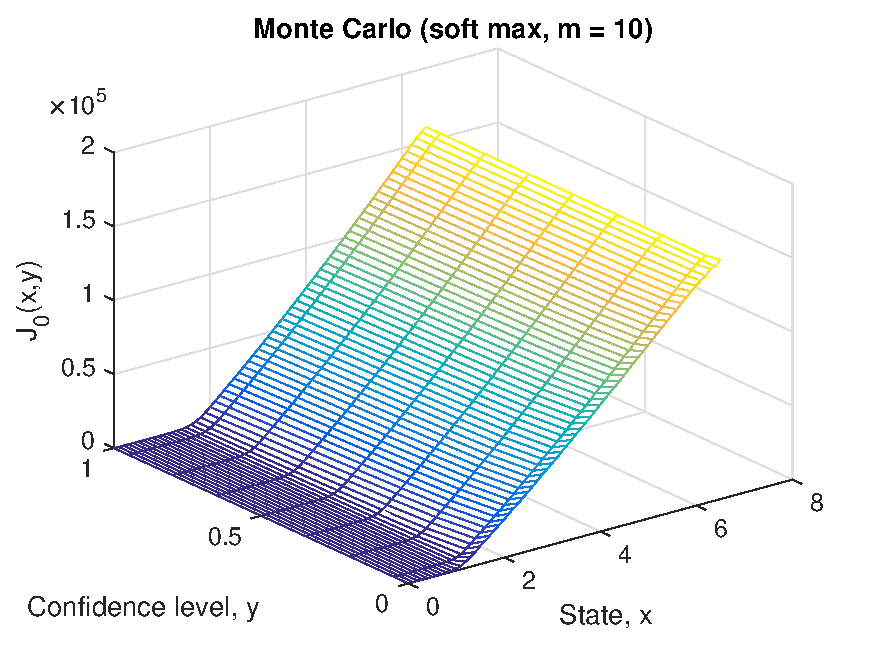
\includegraphics[scale=0.5]{monte_carlo_sum_sept112018.pdf}
      \caption{A Monte Carlo estimate of $J_0^*(x,\alpha)$ versus $(x, \alpha) \in G$ is shown for the pond system, see~\eqref{J0}.
	  $c(x) := \beta e^{m g(x)}$, $\beta := 10^{-3}$, $m := 10$, $\mathcal{K} := [0, 5\text{ft})$, and $g(x) := x-5$.
	  100,000 samples were generated per grid point. See also Fig.~\ref{J0dp}.}
      \label{J0mc}
\end{figure}

\section{Conclusion}\label{conc}
In this paper, we propose the notion of a risk-sensitive safe set and provide a value-iteration algorithm 
that computes an under-approximation. We illustrate our method on a pond system that must be designed to operate safely 
in the presence of uncertain rainfall. Our results suggest that the current pond parameters (e.g., value of the surface area) are 
not sufficient to withstand the design storm. Indeed, keep filling in... 

-inform the cost-effective design of infrastructure that must withstand rare extreme storms,
-possible other applications: to reduce overly conservative error bounds that arise in safe dynamic motion planning (e.g.,~\cite{herbert2017fastrack}), 
and to increase the amount of time that an autonomous vehicle can operate safely while simultaneously optimizing for performance.

%every state contained in the risk-sensitive safe set that we will define enjoys a probabilistic safety guarantee, to be discussed in Sec.~\ref{lemmaconnection}. 
%We are interested in developing a framework for risk-sensitive reachability theory to inform decision-making in an uncertain world, where it may not be sensible to ensure safety by assuming worst-case circumstances.
% Want to quantify varying degrees of safety in a way that realistically (rather than pessimistically) appreciates/prepares for low-probability extreme events through the use of a financial risk measure (i.e., a ``robustified" expected value).
%Computing safe sets under the assumption of worst-case rainfall (e.g., via minimax reachability formulations) is impractical due to the limits of public resources.



\section*{ACKNOWLEDGMENT}
We thank Sumeet Singh, Mo Chen, and Murat Arcak for discussions.
M.C. is supported in part by a NSF Graduate Research Fellowship.
This work is supported in part by NSF CPS 1740079.

\section*{APPENDIX}\label{appendix}
Here we provide the proof of Theorem~\ref{thm}. \textcolor{blue}{please fill in}

\addtolength{\textheight}{-2cm}   % This command serves to balance the column lengths
                                  % on the last page of the document manually. It shortens
                                  % the textheight of the last page by a suitable amount.
                                  % This command does not take effect until the next page
                                  % so it should come on the page before the last. Make
                                  % sure that you do not shorten the textheight too much.

\bibliography{references}

\end{document}
